\documentclass{article}
\usepackage{graphicx}
\usepackage{float}
\usepackage{amssymb}
\usepackage{amsmath}
\usepackage{mathrsfs}
\usepackage{bm}
\usepackage{mathtools}
\usepackage{fullpage}
\usepackage{wrapfig}
\usepackage{hyperref}

\newcommand{\norm}[1]{\left\lVert#1\right\rVert}

\begin{document}

\title{Model Outline}
\author{Octav Dragoi}

\maketitle

\section{Introduction}

The problem is stated as a \textbf{molecule optimization} problem: given one molecule, we wish to come up with another one that improves on certain desirable metrics.

The dataset consists of $N$ pairs of molecules from the set of all molecular graphs $\mathcal{G}$, one being the improved version of the other:
\begin{equation}
    \label{eq:problem_setup}
    D = \{(\mathcal{X}_i, \mathcal{Y}_i) : \mathcal{X}_i, \mathcal{Y}_i\in \mathcal{G}, 1\leq i\leq N\}
\end{equation}

Our model will employ the following components:
\begin{itemize}
    \item A \textbf{Graph Convolutional Network (GCN)}, learning Wasserstein node embeddings in $\mathbb{R}^d, d\in \mathbb{N}$. This takes the shape of a parametric function $G$:
    \[G:\mathcal{G} \rightarrow \mathscr{D}_2({\mathbb{R}^d}),\quad G(\mathcal{X})\in \mathbb{R}^{|\mathcal{X}|\times d} \] 
    where $\mathscr{D}_2({\mathbb{R}^d})$ is the space of all finite point clouds in $\mathbb{R}^d$.
    \item A nonparametric \textbf{tangent space embedding} $\phi = \phi_{Z_0}$ taking a reference point cloud $Z_0\in \mathbb{R}^{N\times d}$. This function, described in \cite{kolouri2020wasserstein}, has the form:
    \[\phi : \mathscr{D}_2({\mathbb{R}^d}) \rightarrow \mathbb{R}^{N\times d}\]
    \item A pseudoinverse \textbf{decoding function} $F\sim G^{-1}$.
    \[F : \mathscr{D}_2({\mathbb{R}^d})\rightarrow \mathcal{G}\]
\end{itemize}

\section{Training}
Given a graph $\mathcal{X}$, the model should learn an improvement direction $\Delta(\mathcal{X})$. We define this direction as:
\[\Delta(\mathcal{X}_i) = \phi(G(\mathcal{Y}_i))-\phi(G(\mathcal{X}_i)) \]

In other words, we encode the graphs $\mathcal{X}_i, \mathcal{Y}_i$ using the GCN, and then project these encodings onto the tangent space at $Z_0$. The difference between these tangent space vectors contains the information on how to modify one vector to obtain the other, and this is what the model should learn.

\begin{figure}[h!t]
    \label{fig:train}
    \begin{center}
        \includegraphics[page=2,width=\textwidth, trim=0 40cm 0 0 ,clip,angle=0]{images/model_outline_train.png}
        \caption{Training flow. Parametrize $\Delta(\mathcal{X}_i)$ in terms of $\mathcal{X}_i$. Only parametric step is the GCN $G$.}
    \end{center}
\end{figure}


The order of the embeddings within $\mathbb{R}^{N\times d}$ is induced by the order we set on $Z_0$, and should not affect the overall modeling process.

From \cite{kolouri2020wasserstein}, $\phi(X) - \phi(Y)\sim W_2(X,Y)$. The quality of this approximation depends on $Z_0$, and therefore $Z_0$ should be picked in an appropriate manner to minimize the approximation error.

\section{Inference}
With the information from $\mathcal{X}$ and $\Delta(\mathcal{X})$, the model should be able to decode $\hat{\mathcal{Y}}$. We define the following:

\[\hat{\mathcal{Y}_i} = F\left(\phi^{-1}\left(\Delta(\mathcal{X}_i) + \phi\left(G(\mathcal{X}_i)\right)\right)\right)\]

Referring to \cite{kolouri2020wasserstein}, $\phi$ is pseudoinvertible, therefore $\phi^{-1}$ should be reasonably well defined.

\begin{figure}[h!t]
    \label{fig:infer}
    \begin{center}
        \includegraphics[page=2,width=\textwidth, trim=0 40cm 0 0 ,clip,angle=0]{images/model_outline_infer.png}
        \caption{Inference flow. Get the $\Delta(\mathcal{X}_i)$ vector from the trained model, add it to the current embedding and then decode.}
    \end{center}
\end{figure}

\section{Open Questions}
\begin{itemize}
    \item The theory around $\phi$ is scarce. How good is the approximation $\phi(X) - \phi(Y)\sim W_2(X,Y)$? How accurate is the pseudoinverse $\phi^{-1}$?
    \item How to write the decoder $F$? Pani and I have a few ideas, but nothing too clear for now.
    \item How to encode the transition from $\mathcal{X}_i$ to $\mathcal{Y}_i$? The difference between tangent vectors is natural, but maybe we can do something fancier with those vectors.
\end{itemize}

\bibliographystyle{ieeetr}
\bibliography{thesisbib}

\end{document}